\documentclass[a4paper,12pt]{article}
%For links
%\usepackage{url}
%For images
\usepackage{graphicx}
%For the "If, else" statment
\usepackage{amsmath}
\begin{document}
\begin{enumerate}
      \item Jag vägde alla mina fyra suddigumm samt en träkub
            och la dom på en 20cm linjal, vilket skulle göra det enkelt
            att mäta distanser. Jag placerade dom som följande:

            Kuben lades -1 cm från mitten och vägde 38.0 gram.
            Sudd 1 lades -6 cm från mitten och vägde 19.2 gram.
            Sudd 2 lades -3 cm från mitten och vägde 15.5 gram.

            Då blir vridmomentet runt -200, vilket måste balanseras på andra sidan.
            Då tog jag mina större sudd.

            Sudd 3 lades 5 cm från mitten och vägde 26 gram.
            Sudd 4 lades 3.6 cm från mitten och vägde 19.2 gram.

            Vridmomentet på höger sida blir då runt 200.
            Med lite småsjusteringar blev det jämnvikt.

      \item
            Följande bild och beskrivning finns i en Volvo V70 instruktionsbok:
            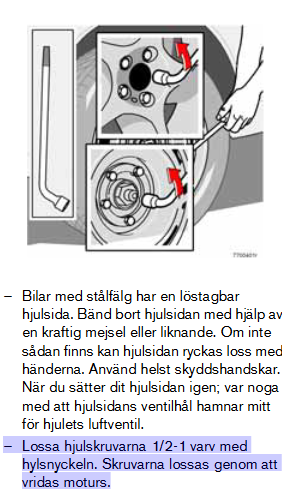
\includegraphics{Figur.png}

            Denna instruktion handlar om hur man lossar på ett hjul, men samma principer
            kan gå åt motsatt håll när man försöker dra åt
            Hylsnyckelns längd kan uppskattas till några decimeter, vi säger 2. Då gäller det att vrida
            bulten 1 varv, vilket krävs för att dra åt den helt.

            Då blir hävarmen runt 2 gånger kraften som man drar med. Ju hårdadre man drar destå
            mer hävarm.

      \item Det antas att $y_0=0$ och det ska tas reda på när y blir 0.
            $$0=tvsin(\alpha)-\frac{gt^2}{2} \Rightarrow t=\frac{2vsin(\alpha)}{g}\approx 2$$

            Den högsta punkten är vid t/2 eftersom att parabolen som bildas är symmetrisk när
            man avfyrar från marken.

            $$v_y=v_0sin(\alpha)-g(t/2) \Rightarrow v_y=0$$

            Vid kastbanans högsta punkt så är alltså hastigheten för y axeln 0. Detta är för att
            kulan är precis vid sin maxpunkt och är påväg att börja åka neråt på grund utav
            graviationskraften.

            Istället kan endast hastigheten på x-axeln räknas ut enkelt så här:
            $22*cos(27^\circ)=20 m/s$ vilket då också är den totala hastigheten vid den punkten.

      \item
            För att simplifiera problemet kan man vinkla flaggstången så den liknar
            en gungbräda. Då får vi följande diagram:

            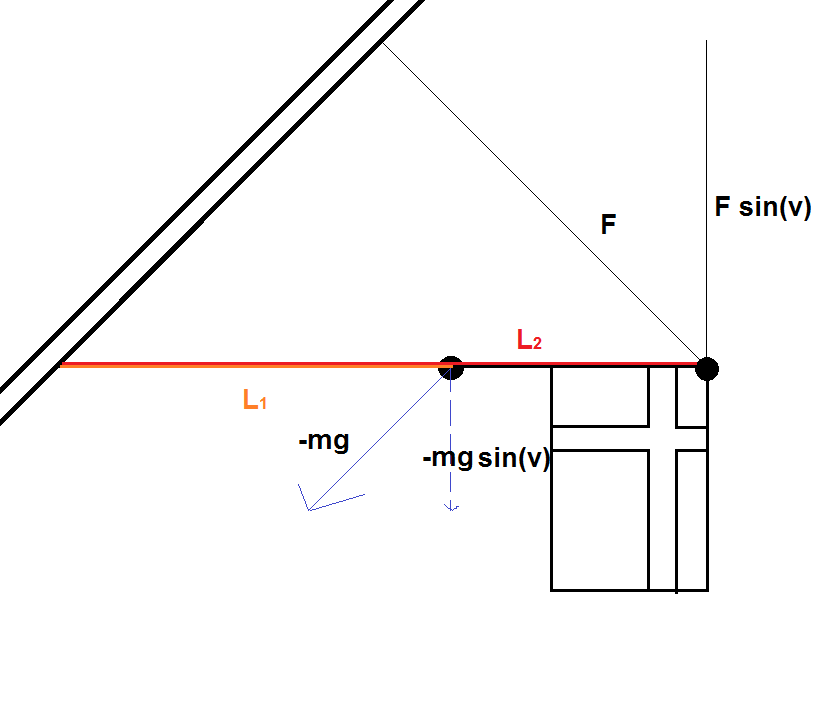
\includegraphics[scale=0.55]{Figur2.png}

            Flaggstången är i jämnvikt, så genom momentlagen får vi att summan av vridmomenten
            blir noll.

            $$FL_2sin(v)-mgL_1sin(v)=0$$
            $$FL_2=mgL_1$$
            $$F==\frac{mgL_1}{L_2}$$

            I uppgiften får vi reda på att massan på flaggstången är 53kg, Längden till
            tyngpunkten är 5 meter från punkten och att hela flaggstångens längd
            är 8.4 meter. Då får vi att F = 310 N.

      \item

            Man kan se att från perspektivet av Peter så accelererar myntet
            med motsatt acceleration som bussen.

            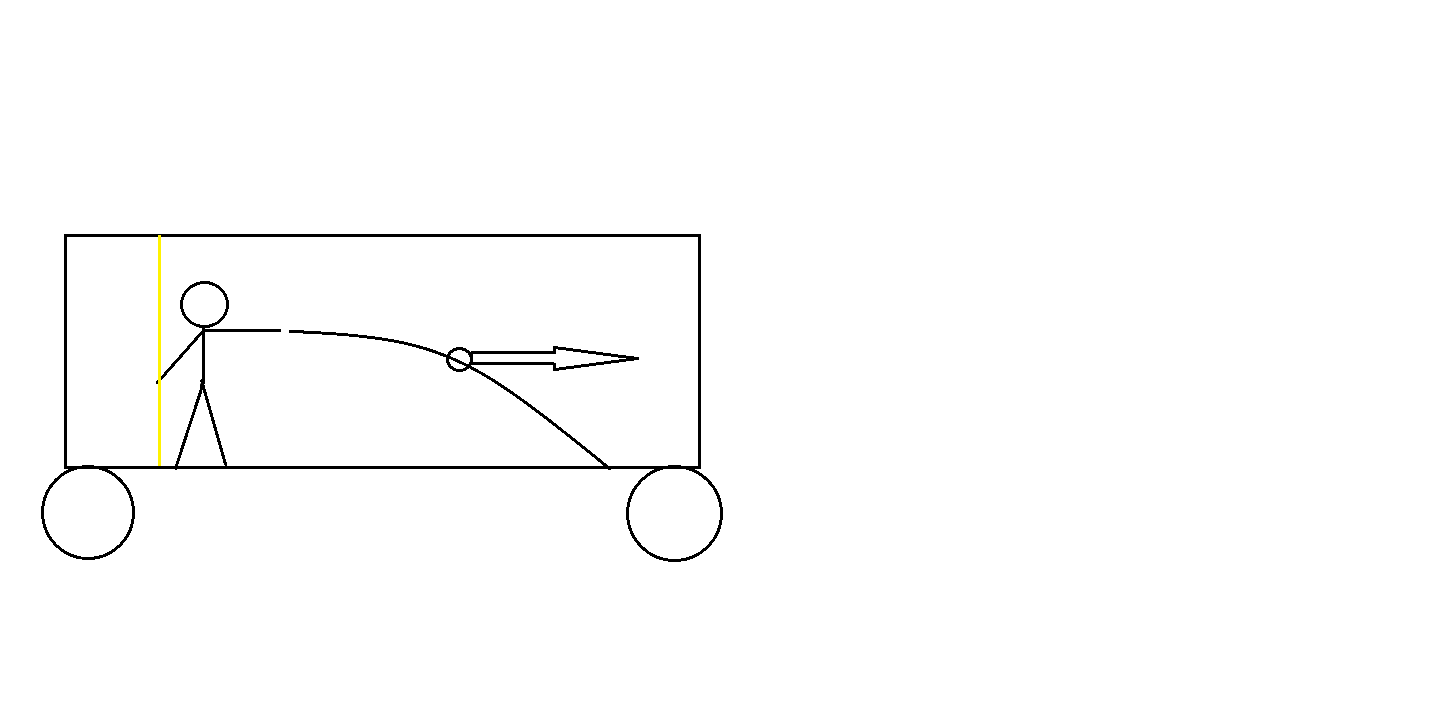
\includegraphics[scale=0.5]{Figur3.png}

            Då får vi att bollens x-position är

            $$x=x_0+v_{x0}t+\frac{1}{2}at^2$$

            Men vi antar att $x_0=0$.
            Ekvationen simplifieras då till

            \begin{equation}
                  x=v_{x0}t + \frac{1}{2}at^2
            \end{equation}

            Variabln som bör räknas ut är då t.
            Detta kan räknas ut i y-dimensionen där gravitationskraften
            drar ner myntet till golvet under en viss tid.

            $$y=y_0-\frac{1}{2}gt^2$$

            Den tiden det tar att landa på marken är när y=0,
            och ekvationen kan då skrivas om som

            \begin{equation}
                  t=\sqrt{\frac{2y_0}{g}}
            \end{equation}

            Då sätts t från ekvation (2) in i ekvation (1)

            $$x=v_{x0}\sqrt{\frac{2y_0}{g}} + \frac{1}{2}a\sqrt{\frac{2y_0}{g}}^2$$
            $$x=v_{x0}\sqrt{\frac{2y_0}{g}} + a\frac{y_0}{g}$$

            Med $a=-2.3$, $g=9.81$, $v_{x0}=25$ och $y_0=1.5$ får man att
            myntet faller 13.48 meter bort. Men det finns anledningar
            till att tro att den skulle åka längre i verkligheten, för
            objekt kan studsa, rulla och glida, vilket dom här
            ekvationerna inte täcker.

\end{enumerate}
\end{document}